%!TEX root = ../../thesis.tex
\section{Adaptive control}
\noindent As briefly discussed in the introduction, the dynamics model will be used as a control-oriented framework for model-based controllers applicable to soft robotics. In retrospect to previous model-based controllers, Della Santina et al.  \cite{DellaSantina2020} proposed a combination of feedforward and model-based feedback; yet, satisfying the passivity condition, more robustness approach could be acquired through energy-based controller (especially in the face of material uncertainties). Franco et al. \cite{Franco2020} proposed an adaptive energy-based controller but the underlying model (multi-link pendulum) is not rooted in a continuum description. Here, we wish to provide a mix of the control methodologies -- an energy-based control approach for the continuous PCC model with an adaptive material law.
%
\subsection{Passivity-based adaptive control}
\noindent The continuous dynamics of the soft robotic manipulator are described by \eqref{eq:C2:dynamic_model}, where the Lagrangian system matrices depend on physical parameters, e.g., mass, moments of inertia, stiffness, and viscosity. Within the context of robust control, these parameters often deviate from their true value. So merely an estimate of the system matrices $\tmat{M}(\q)$, $\tmat{C}(\q,\q)$, $\tvec{f}\!\grav(\q)$ and $\tvec{f}\!\elastic(\q,\dq)$ can be acquired, where we denote $
\Delta (\cdot) = \tilde{(\cdot)} - (\cdot)$ as the difference between the true value and its estimate. The difference (or uncertainty) between true and estimated values is of particular relevance in soft robotics, where material properties play a significant role on both the statics and dynamics. Poor estimates of the material parameters could lead to instability in some model-based controllers if not considered carefully. Exploiting the passivity in Lagrangian models, we can derive a passivity-based adaptive controller similar to the works of Slotine et al. \cite{Slotine1988} and Ortega et al. \cite{Ortega1998}. The benefit of passivity-based control techniques is its robustness regarding parameter uncertainties and unmodelled dynamics. Passivity-based control is rooted in energy-shaping and damping injection techniques, leading to simple implementation yet effective means of stabilization.
%

Let $\q_d \in \mathcal{Q}$ be the desired trajectory of the soft robot together with its time-derivative $\dq_d,\ddq_d \in {\R^n}$. Next, let $\piB \in \mathbb{R}^p$ be a vector containing all unknown values from a set of physical parameters, and the parametrization error $\vec{e}_{p} := \vec{\tilde{\piB}} - \piB$ in which the the vector $\vec{\tilde{\pi}} \in \R^p$ denotes the parameter estimates. \editl An important note is that the model must be linear in $\piB$, which holds true for the line-density $\rho_0$, the linear elasticity parameters in \eqref{eq:C2:stiffness_tanh_beta} and \eqref{eq:C2:stiffness_tanh_eps}, damping, creep coefficients in \eqref{eq:C2:creepmodel} and \eqref{eq:C2:creepcompliance}, and also for an unknown mass applied at the tip of the soft robot \eqref{eq:C2:delta_payload}. Unfortunately, we cannot included the material parameters $\alpha_3$  and $\alpha_6$ due to their nonlinear dependence.\editr The control objective is given by finding an appropriate control input and update law such that $\lim_{t\to \infty} \q(t) = \q_d(t)$ is achieved with good transient behavior. Assuming linearity in the parameters
% Linearity in parameters holds true for the line-density $\rho(q,\sigma)$ and all linear visco-elastic stiffness constants. As such, the nonlinear parameters $\alpha_3$ and $\alpha_6$ cannot be included into the estimation law.},
the linear parametrizability matrix of the soft robot's dynamics is given as follows
%
\begin{equation}
\vec{Y}(\cdot,\piB)\,{\vec{e}_p} = \Delta \mat{M}\,\ddq_r + \Delta \mat{C}\,\dq_r + \Delta \vec{f}\grav +  \Delta\vec{f}\elastic +  \Delta \vec{\delta},\label{eq:regress}
\end{equation}
%

\begin{figure}[!t]
    \vspace{-0.6mm}
    \centering
    %%!TEX root = ../../thesis.tex
%%%% CHAPTER 1 *****************************************************************
\chapter[Dynamic modeling of Soft Robots -- PCC case]{Dynamic modeling -- The Piece-wise Constant Approach}
\label{chap: chapter 1}

\blankfootnote{This chapter is based on:\\ .\disclaimer}

%%%% ABSTRACT ******************************************************************
%!TEX root = ../../thesis.tex
\chapterabstract{The motion complexity and use of exotic materials in soft robotics call for accurate and computationally efficient models intended for control. To reduce the gap between material and control-oriented research, we build upon the existing Piecewise-Constant Curvature framework by incorporating hyper-elastic and visco-elastic material behavior. In this work, the continuum dynamics of the soft robot are derived through the differential geometry of spatial curves, which are then related to Finite-Element data to capture the intrinsic geometric and material nonlinearities. To enable fast simulations, a reduced-order integration scheme is introduced to compute the dynamic Lagrangian matrices efficiently, which in turn allows for real-time (multi-link) models with sufficient numerical precision. By exploring the passivity and using the parametrization of the hyper-elastic model, we propose a passivity-based adaptive controller that enhances robustness towards material uncertainty and unmodeled dynamics -- slowly improving their estimates online. As a study case, a fully 3D-printed soft robot manipulator is developed, which shows good correspondence with the dynamic model under various conditions, e.g., natural oscillations, forced inputs, and under tip-loads. The solidity of the approach is demonstrated through extensive simulations, numerical benchmarks, and experimental validations.}


%%%% MAIN **********************************************************************
\section{Introduction} \label{sec: chap1 1_introduction}
%!TEX root = ../../thesis.tex
The field of soft robotics has attracted the interest of many researchers from different backgrounds. Soft robots use compliant and hyper-elastic materials, while the use of rigid materials is minimized. The introduction of soft materials into robotics greatly expanded the field of application for robotics. For example, due to their dexterity and environmental robustness, soft robots are often used in medical applications \cite{Polygerinos2015b, Yap2015, Asbeck2015}, adaptive grasping \cite{Galloway2016, Hughes2016}, and locomotion in uncertain environments \cite{Drotman2017}. Unlike its rigid counterpart, soft robots undergo large continuum-bodied motion that, to some extent, resembles morphologies found in nature. These morphologies arise by virtue of the low compliance in soft materials and, more importantly, the structural layout of the soft robot. As of today, many of the fundamental engineering principles in rigid robotics, like design, actuation, sensing, and control, are often not applicable to soft robotics systems. Since its inception, most of these engineering problems have remained challenging or unresolved.

Although the diversity in soft robotics is significant, ranging from adaptive grippers to soft manipulators, most topologies in soft robotics can be associated with nature or engineered geometries for minimal compliance (e.g., bellow shapes). Soft robots often mimic living creatures and their morphologies, e.g., the tentacle of an octopus \cite{Galloway2016, Wehner2016}, or the trunk of an elephant \cite{Drotman2017}. Hypothetically, the abundance of bio-mimicry in soft robotics might be associated with the design complexity of developing robots from soft materials. The large number of degrees-of-freedom and exotic mechanical nature of soft robots makes design significantly challenging, and consequently, the design process can be iterative and time-consuming \cite{Wehner2016}. Therefore, it becomes potentially advantageous to use computational tools that assist or develop appropriate soft robotic topologies given a set of user-defined requirements, like desired motion or force.

In the past, researchers have made efforts to finding morphologies through mathematics, in particular through evolutionary algorithms. The concept of automated creature designs was first introduced by Sims \cite{Sims1994}, who showed that, given a set of basic geometries, locomotive organisms could be generated from evolutionary algorithms. These virtual organisms resembled biological morphologies to some extent; however, the complexity of the material layout was limited. More recent work involving the synthesis of virtual soft robots includes Cheney et al. \cite{Cheney2013}, who successfully produced intricate locomotive morphologies using artificial neural networks and multi-material parameter spaces of active and passive soft voxels. Other work involving morphological synthesis includes \cite{Bern2019, Morzadec2019,Diepen2019}. Unfortunately, the synthesis of morphologies from previous approaches, though novel, remains only in ideal simulated environments. An accurate representation of the nonlinear material properties in soft robotics can be challenging, and in favor of computational efficiency, little detail is spent on the nonlinear nature governing soft materials. Besides, these evolutionary frameworks typically involve a network of `activation' cells or voxels that perform ideal volumetric deformation, biologically resembling muscle functionality while unfortunately lacking resemblance to conventional actuation in soft robotics, e.g., pneumatics, dielectrics, and smart metal alloys (SMA).

Reviewing previous methods, a more efficient approach for solving the optimal morphology might be founded in topology optimization. Topology optimization is the general formulation of a material distribution problem for mechanical solids, where density-based topologies arise throughout an iterative (non-convex) optimization procedure. The synthesis of compliant mechanisms through topology optimization is investigated thoroughly \cite{Sigmund2015, Gain2013, Luo2015}; however, its application to soft robotics is relatively unexplored \cite{Zhang2018,Zolfagharian2019}. Yet, to obtain meaningful topologies for soft robotics, two problems need to be addressed. Since soft robots undergo large deformations, it becomes necessary to describe the nonlinear geometrical deformations accurately. Inherent to significant deformation of soft materials is the importance of nonlinear material behavior, like hyperelasticity. Another concern is the design-dependency of the external forces, in our case, the pneumatic loads. This class of structural problems is more challenging than traditional problems since the load is continuously interacting with the adaptive interface during the iterative optimization process \cite{Wang2016, Vasista2013}. It should be mentioned that the use of compressed air or pressurized fluid is a popular actuation approach in soft robotics.

In this work, we present a novel framework for generating topologies of soft robotics. Contrary to biometry or convectional designs, finding the (optimal) material layout of the soft robot is accomplished through a gradient-based nonlinear topology optimization, where the distribution of soft materials is optimized given a user-defined objective. Our main contributions include the description of nonlinear geometrical deformation and pneumatic loading. We exploit the connectivity properties in polygonal meshes such that synchronized volumetric contraction or expansion of a group of polygonal elements can artificially mimic the geometrical loads in pneumatic actuation. The advantages of our framework in comparison to other literature are: ($i$) a better representation of pneumatic actuation in soft robotics; ($ii$) improved design convergence in contrast to evolution-based optimization methods. To our knowledge, our approach of pressure-driven nonlinear topology optimization is new for soft robotics, and its application could easily extend to other soft robotic systems. %The computational framework detailed in this work is made publicly available at \cite{Caasenbrood2019}.

The remainder of the paper is structured as follows. In section \ref{chap:fem}, we will discuss the continuum mechanics for hyper-elastic materials, followed by a description of the optimization scheme for soft robotics. In section \ref{chap:results}, we propose a numerical example for developing a soft robotic structure to illustrate the effectiveness of our approach.


\newpage
\section{Continuum dynamic model}  \label{sec: chap2 section header}
%!TEX root = ../../thesis.tex
As mentioned previously, soft robots are composed of soft bodies that may be regarded as a continuum body with (theoretically) infinitely many degrees-of-freedom (DOF). In this section, we aim to derive a compact and computationally efficient model that envelops the continuous dynamics of a soft robot through a small set of generalized coordinates $\q\in\Q$ and their respective generalized velocities \highlight{$\dq(t)\in T_{\q}\Q$} with $n$ the number of active joint variables. We base {the modeling framework on the work of Mochiyama et al.\cite{Mochiyama2003} who outlined a theoretical foundation for continuum manipulators. Their work is extended upon by including extensibility, serial-chaining of multiple soft-links, pneumatic actuation, and the introduction of nonlinear and time-dependent material behavior. Earlier modeling strategies addressing similar issues can be found in from Godage et al. \cite{Godage2015,Godage2016}, Della Santina et al. \cite{Santina2020,Santina2020b,Santina2020Pcc}, Renda et al. \cite{Renda2018}, and Boyer et al. \cite{Boyer2021}. Leveraging from the aforementioned works, the continuous dynamics of a soft robot manipulator can be written in the familiar Lagrangian form:
%
\begin{equation}
\MB(\q) \ddq + \vec{h}(\q,\dq) = \Qnc,
\end{equation}
%
where $\MB(\q)  \in \R^\nn$ denotes the generalized inertia matrix, $\vec{h}(\q,\dq) \in \R^n$ a vector of nonlinear state-dependent force contributions. In this work, a similar modeling framework is adopted; however, we propose an extension to incorporate FEM-driven data to more accurately reflect the underlying continuum mechanics -- in particular hyper-elasticity; and we propose a numerical scheme that allows for fast computation of the continuous dynamics. For completeness, we will recapitulate on the modeling approach here.

\subsection{Kinematics of elastic continuum bodies}
\noindent To represent the hyper-flexible configuration of the soft robot, let us consider a smooth spatial curve that passes through the geometric center of the continuously deformable body, as shown in Figure \ref{fig:configuration}. {In literature, this curve is called} the '\textit{backbone curve}' as it simplifies the three-dimensional deformation imposed by distributed forces acting on the elastic body. The arc-length of the backbone corresponds to the extensible length of the soft robot denoted by the variable $l(t) \in [l_{-},l_{+}]$ which we assume bounded $l_{+} \ge l \ge l_{-}$, and let $L$ be a constant denoting the {total unstressed} length of the soft robot. Next, let us introduce a spatial variable
$\sigma \in \Xs$ that belongs to the one-dimensional material domain of the backbone curve, i.e., $\Xs = [0,\, L]$. {Let it be clear that the spatial variable $\sigma$ represents the arc-length of a material coordinate along the undeformed material domain of the soft robot manipulator.}

\commentary{}{Figure here of smooth curve for p and Phi}

Given each material coordinate, we wish to find a suitable low-dimensional joint representation $q(t)$ such that the position vector $^0p$ anywhere on the continuous backbone can be written as a mapping from generalized coordinates and space into $\mathbb{R}^3$:
%
\begin{equation}
^0\pB: \Xs \times \Q(t) \to \R^3;
\end{equation}
%
and similarly the rotation matrix $^0\mat{\Phi}(\sigma,\vec{q})$ by a mapping from the generalized coordinates and space into $\SO{3}$:
%
\begin{equation}
^0\PhiB: \Xs \times \Q(t) \to \SO{3}, \label{eq:phi_map}
\end{equation}
%
where {$\SO{3}$ denotes the special orthogonal group for rotations about the origin of $\R^3$}, and $n = \dim(\vec{q})$ the state dimension. Under this notion, the position vectors $^0p(q,0)$ and {$^0\pB(L,\q)$} relate to the base and the end-effector of the soft robot, respectively. {Please note that left-sided superscript are used to indicate the frame of reference.} The set of all points on the backbone $\mathcal{P} = \left\{^0\pB \in \R^3\, |\, \sigma \in \Xs \right\}$ draws a possible {spatial} configuration of the soft robot given {a time instance $t \in \mathbb{T}$ on a finite horizon $\mathbb{T} = [0,T]$}.
%
\begin{intermez}
Despite the inherent flexibility in soft robotics, it is sometimes sufficient to express the kinematics according to the Piecewise Constant Curvature (PCC) condition. Mathematically, it implies that the curvature of the continuous body satisfies $\kappa(q,\sigma_1) = \kappa(q,\sigma_2)$ for a neighboring region of points $\sigma_1,\sigma_2 \subseteq \Xs$. As a result, this condition allows us to describe the full forward kinematics with a significantly reduced set of generalized coordinates, mitigating kinematic complexity in the model. Numerous works employ PCC models \cite{Falkenhahn2015,Katzschmann2019,Tatlicioglu2007,Marchese2016,Godage2016,Santina2020Pcc}, and depending on the degrees of elasticity, the PCC condition has been proven to be consistent for various soft robotic systems.
\end{intermez}
%
{Following this Piecewise Constant Curvature (PCC) description, let us assign a coordinate frame that twists minimally along the backbone -- a Bishop frame \cite{Bishop1975}-- parametrized by the following generalized coordinate vector:}
%
\begin{equation}
\vec{q} = \begin{pmatrix}
\,\varepsilon & \kappa_x & \kappa_y\,
\end{pmatrix}^\top \in \mathcal{Q},
\label{eq:coordinate}
\end{equation}
%
\noindent where {$\varepsilon \in \R$ is the elongation strain}, and $\kappa_x,\,\kappa_y\in\mathbb{R}$ are the curvatures or angular strains in $x$-$z$ and $y$-$z$ plane, respectively; and $\mathcal{Q} \subset \R^3$ is an admissible space on which $q$ evolves.It is worth mentioning that the joint description above is somewhat related to Renda. et al. \cite{Renda2018} who proposed a Piece-wise Constant Strain (PCS) parametrization with the exception of including the twist along the tangent.

By exploring the differential geometry of the smooth backbone curve similar to Mochiyama et al.\cite{Mochiyama2003}, we can express the spatial change of the position vector $^0 \vec{p}(0,\vec{q})$ and the orientation matrix $^0\mat{\Phi}(q,\sigma)$ for each material point $\sigma$ along the smooth backbone by
%
\begin{align}
\renewcommand*{\arraystretch}{2}{}
\frac{\partial \,^0\!\mat{\Phi}}{\partial \sigma}(\sigma,\vec{q}) & = \, ^0\mat{\Phi}(\sigma,\vec{q})\,\left[\mat{\Gamma} (\sigma,\vec{q}) \right]_{\times}, \label{eq:change_phi} \\
\frac{\partial \,^0\! \vec{p}}{\partial \sigma}(\sigma,\vec{q}) & = \, ^0\mat{\Phi}(\vec{q},\sigma) \, \vec{U}(\sigma,\vec{q}), \label{eq:change_p}
\end{align}
%
where $[\vec{\Gamma}]_\times \in \So{3}$ is a skew-symmetric matrix composed of the entries of the vector $\vec{\Gamma} \in \R^3$, and $\vec{U}\in \R^3$ a vector representing the tangent along the extensible backbone. The vectors $\vec{\Gamma}$ and $\vec{U}$ are vectors that define the differential geometry of the backbone, which are unique entries that lives in the tangent space of the rigid-body transformation group $\SE{3}$. Given the Bishop parametrization as described by \eqref{eq:coordinate}, these geometric entities yield
%
\begin{equation}
\vec{\Gamma} = \begin{pmatrix} -\kappa_y \\ \kappa_x \\ 0  \end{pmatrix}; \quad \quad \quad \vec{U} = \begin{pmatrix} \,\, 0 \,\, \\ \,\, 0 \,\, \\ \, \,\varepsilon \,\, \end{pmatrix} + \vec{U}_0,
\end{equation}
%
with $\vec{U}_0 = (0,0,1)^\top$ the unit-tangent. Now, given an initial configuration of backbone's base, i.e., $^0 \mat{\Phi}(0,\vec{q}) = \vec{\Phi}_0$ and $^0 \vec{p}(0,\vec{q}) = 0_3$, we can now solve for the position and orientation for each material coordinate $\sigma$ along the backbone:
%
\begin{align}
^0\mat{\Phi}(\sigma,\vec{q}) & = \vec{\Phi}_0\exp(\sigma [\vec{\Gamma}(\vec{q})]_\times), \label{eq:phi_exact} \\
^0\vec{p}(\sigma,\vec{q}) & = \int_0^\sigma\,^0\mat{\Phi}(\eta,\vec{q})\, \vec{U}(\vec{q}) \; d\eta, \label{eq:pos_vector}
\end{align}
%
where $\exp: \So{3} \to \SO{3}$ is the exponential map. Let it be clear that the closed-form solutions \eqref{eq:phi_exact} and \eqref{eq:pos_vector} form the forward configuration kinematics of the backbone curve. To express the forward velocity kinematic, let  $\vec{V}(\sigma,\vec{q},\dot{\vec{q}}) = \left(^\sigma \vec{\omega}^\top,^\sigma \vec{v}^\top \right)^\top \in \R^6 \cong \Se{3}
$ be the aggregate of the angular velocity and linear velocity components relative to an inertial frame at $\sigma$ (the frame of reference is denoted by a left superscript), where the space $\Se{3}$ denotes the Lie algebra of $\SE{3}$. The velocity twist is computed by the following integration procedure:
%
\begin{equation}
 \vec{V}(\sigma,\vec{q},\dot{\vec{q}}) = \Ad_{\mat{g}(\sigma,\cdot)}\inv \int_0^\sigma \Ad_{\mat{g}(\eta,\cdot)}\, J^*\! \dot{q}\;d\eta
 \,=:\, J(q,\sigma) \dot{q}, \label{eq:vel_cont}
\end{equation}
%
where $\Ad_g: \SE{3} \to \mathbb{R}^{6\times 6}$ denotes the adjoint transformation matrix regarding the rigid body transformation $g \in \SE{3}$ that maps local velocities (i.e., twist) to a frame located at $\sigma$, and $J^*$ a constant joint-axis matrix. The joint-axis matrix for an extensible and bendable PCC segment parametrized by the Bishop parameters is given by
%
\begin{equation}
\renewcommand*{\arraystretch}{1}{}
J^* := \left(\dfrac{\p \Gamma}{\p q}^\top \; \dfrac{\p U}{\p q}^\top \right)^\top  = \begin{pmatrix}
\,0 & 0 & 0 & 0 & 0 & 1 \, \\
\,0 & 1 & 0 & 0 & 0 & 0 \,  \\
\,-1 & 0 & 0 & 0 & 0 & 0 \,  \\
\end{pmatrix}^\top. \label{eq:joint-axis-matrix}
\end{equation}
%
Although we based the forward kinematics on the work of Mochiyama et al.\cite{Mochiyama2003}, the derived expression for the velocity twist in \eqref{eq:vel_cont} is analogous to the work of Renda et al.\cite{Renda2018,Renda2020}, and Boyer et al. \cite{Boyer2010,Boyer2021}. Please also note that \eqref{eq:vel_cont} gives rise to the geometric manipulator Jacobian $J(q,\sigma)
$ that defines the mapping from joint velocities to the velocity twist for a particular material point $\sigma$ on the continuous body. In continuation, let us also introduce the acceleration twist\cite{Boyer2021,Mochiyama2003,Renda2018} -- obtained through time differentiation of \eqref{eq:vel_cont}:
%
\begin{align}
\dot{V}(q,\dot{q},\ddot{q},\sigma) & = J \ddot{q} + \Ad_{g(\cdot,\sigma)} \inv \int_0^\sigma \Ad_{g(\cdot,\eta)}
\ad_{V(\cdot,\eta)} \, J^*\! \dot{q}\;d\eta \notag \\
& := J(q,\sigma)\ddot{q} + \dot{J}(q,\dot{q},\sigma) \dot{q},
\label{eq:acceleration}
\end{align}
%
where $\ad_{V} \in \mathbb{R}^{6\times 6}$ denotes the adjoint transformation regarding the velocity twist $V \in \Se{3}$. The reader is referred to Appendix A for more detailed expressions on the adjoint transformations.
%
\subsection{Euler-Lagrange equations}
\noindent Given the forward kinematics in \eqref{eq:phi_exact}, \eqref{eq:pos_vector}, \eqref{eq:vel_cont} and \eqref{eq:acceleration}, we can shift our attention to formulating the finite-dimensional dynamics of the soft robot. Our goal here is to write the spatio-temporal dynamics of the hyper-elastic soft robot as a second-order ODE into the Lagrangian form:
%
\begin{equation}
\frac{d}{d t}\left(\frac{\partial \mathcal{L}}{\partial \dot{{q}}}\right) - \frac{\partial \mathcal{L}}{\partial {q}} = {Q}^{\nc}, \label{eq:euler_largrange}
\end{equation}
%
\noindent where $\La({q},\dot{q}) := \T(q,\dot{q}) - \mathcal{U}(q)$ is the Lagrangian function, $\T \in \Rp$ and $\mathcal{U}\in \R$ the kinetic and potential energy, respectively; and $Q^{\nc} \in \mathbb{R}^n$ a vector of generalized non-conservative forces. To apply the Lagrangian formalism to a continuum dynamical system, regard an infinitesimal slice of the continuum body for each material coordinate $\sigma$ along the backbone curve. Given this notion, we embody this infinitesimal slice with an inertia tensor $
\mathcal{M} = \text{blkdiag}(\rho I_3,\mathcal{J_\sigma})$ with $\rho = m/L$ the line-density and $J_\sigma$ a tensor for the second moment of inertia. The kinetic energy can be obtained through spatial integration of its respective kinetic energy densities\cite{Boyer2010,Mochiyama2003,Tatlicioglu2007}, i.e., $\mathfrak{T} = \frac{1}{2}V^\top \mathcal{M} V
$:
%
\begin{align}
\mathcal{T}({q},\dot{{q}}) & = \frac{1}{2}\int_\Xs {V}({q},\dot{q},\sigma)^\top\,\mathcal{M}\,{V}({q},\dot{{q}},\sigma) \; d \sigma,
 \notag \\
& =  \frac{1}{2} \dot{q}^\top \int_\Xs  J({q},\sigma)^\top\,\mathcal{M}\, J({q},\sigma) \; d \sigma \, \dot{q}, \notag \\
& = \frac{1}{2}\dot{q}^\top M(q) \dot{q}. \label{eq:kinetic_energy}
\end{align}
%
Note that expression for the kinetic energy naturally gives rise to the generalized inertia matrix $M(q)$ of the Lagrangian model. By substitution of the kinetic energy into the Euler-Lagrange equation \eqref{eq:euler_largrange}, we find $M(q)\ddot{q} + C(q,\dot{q})q$ where $C(q,\dot{q})$ denotes the Coriolis matrix. Instead of computing the Coriolis matrix through the conventional Christoffel symbols\cite{Murray1994}, we adopt a computational scheme by Garofalo et al. \cite{Garofalo2013} used for serial-chain rigid manipulators, in which we replaced the finite summation of $N$ rigid-bodies by a spatial integration over the continuum domain $\Xs$:
%
\begin{equation}
C(q,\dot{q}) = \int_\Xs J(q,\sigma)^\top \Ct_{V(q,\dot{q},\sigma)}J(q,\sigma)\; + J(q,\sigma)^\top \Mt \dot{J}(q,\dot{q},\sigma) \; d \sigma,\label{eq:coriolis}
\end{equation}
%
where $\Ct_{V} = -\Ct_{V}^\top :=  \mathcal{M} \ad_{V}  - \ad_{V} ^\top \mathcal{M}$ is a skew-symmetric matrix. The computation above is slight different from existing literature\cite{Boyer2021,Renda2020} to ensure that the matrix $\dot{M} - 2C$ is skew-symmetric; the so-called the passivity condition\cite{Murray1994} for Euler-Lagrange systems (see Appendix B for proof). The importance of this property will become apparent later in the energy-based controller design. Lastly, the potential energy is given by sum of gravitational potential energy and internal elastic potential, i.e., $\mathcal{U}({q}) = \mathcal{U}_g({q}) + \mathcal{U}_e({q})
$. Since gravitational potential energy density is \rewritten{given} by $\mathfrak{U}_g = -\rho\,^0p(q,\sigma) \gamma_g$ with $\gamma_g \in \R^3$ is a vector of body accelerations, the potential energy related to gravity is obtained by spatial integration of their respective energy densities:
%
\begin{equation}
\mathcal{U}_g({q}) = - \rho \int_\Xs \,^0p(q,\sigma)^\top \gamma_g \; d \sigma.
\label{eq:potential_energy_grav}
\end{equation}
%
\noindent To model the hyper-elastic nature, lets introduce two nonlinear stiffness functions for both stretching and bending, denoted by $k_e: \R \mapsto \Rsp$ and $k_b: \R \mapsto \Rsp$, respectively. These functions allow us to describe a collective elastic behavior imposed by the hyper-elastic materials and the continuum-bodied deformation. It shall be clear that these entities are unique to the soft robot's geometry and soft material choice, and thus finding a suitable candidate model requires further analysis. Later, we will sculpt these nonlinear stiffness functions through Finite Element Methods (FEM). For now, we assume that these analytical nonlinear stiffness functions are known, and thus the (hyper)-elastic potential energy takes the form
%
\begin{equation}
\mathcal{U}_e({q}) = \int_0^{\varepsilon} k_e(\eta) \,\eta \; d \eta + \int_0^{\beta(q)} k_b(\eta)\, \eta \; d \eta,
\label{eq:potential_energy_elas}
\end{equation}
%
where $\varepsilon$ is the elongation strain, and $\beta({q}) = \kappa L (\varepsilon + 1)$ is the bending angle with the total curvature of the soft segment $\kappa = \sqrt{{\kappa_x}^2 + {\kappa_y}^2}$ (see Figure \ref{fig:configuration}).
\subsection*{Overall dynamics}
\noindent Finally, by combining \eqref{eq:euler_largrange}, \eqref{eq:kinetic_energy}, \eqref{eq:coriolis}, \eqref{eq:potential_energy_grav}, and \eqref{eq:potential_energy_elas}, the continuum dynamics of the soft robot can be casted into the familiar closed form \cite{Santina2020Pcc,Boyer2021,Renda2018,Godage2016} similar to aforementioned model (1):
%
\begin{align}
M({q})\,\ddot{{q}} + {C}({q},\dot{{q}})\,\dot{{q}} + P({q},\dot{q}) + G({q}) & = \tau(u,\delta), \label{eq:dynamic_model}
\end{align}
%
\noindent where $P = d \mathcal{U}_e/d q + R\dot{q}$ is a vector of generalized forces imposed by the deformation of the soft materials with $R \in \R^{n\times n}$ the Rayleigh damping matrix, $G = \p \mathcal{U}_g/\p q$ a vector of generalized gravitational forces, and $u \in \R^m$ the control input with the index $m$ the number of pressure inputs. The generalized input vector is chosen of the form: $\tau(u,\delta) = H u + \delta$ with $H: \R^m \mapsto \R^n$ a mapping from the input space to the joint actuation space, and $\delta(t)$ an external disturbance (e.g., unmodelled material uncertainties).
%
\begin{rmk}
Given the context of manipulators, a possible disturbance $\delta(t)$ could be an external mass applied to the tip of the soft robot. Given the kinematic relations in \eqref{eq:vel_cont} and \eqref{eq:acceleration}, one can describe the disturbance (modeled here as a point-mass located at $L$) by a state-dependent vector:
%
\begin{equation}
\delta_m = m_\delta \floor{J(\cdot,L)}_3^\top\left({\normalfont \Ad}_{g(\cdot,L)}\inv\gamma_g + \floor{\dot{V}(\cdot,L)}_3 \right),
\label{eq:delta_payload}
\end{equation}
%
where $\floor{\cdot}_3$ extracts the last three rows of a matrix or vector, and $m_\delta > 0$ the applied mass to the end-effector. It is worth recalling that the acceleration twist can be computed through the geometric Jacobian and its time derivative, i.e., $\dot{V} = J\ddot{q} + \dot{J}\dot{q}$. Indeed, the PCC condition for a soft body can only accurately describe the true dynamics if external forces produced by mass $m_\delta$ do not excessively exceed the intrinsic elastic balancing forces $P(q)$. Alternatively, a soft body can be modeled using multiple PCC curves of smaller size, similar to standard Finite Element discretization.
\end{rmk}

The actuation mapping $H$ depends on the geometry, placement, and orientation of the (pneumatic) soft actuators. Since the pneumatic chambers are aligned parallel to the backbone curve and are equally spaced along the circumference, we propose the following ansatz:
%
\begin{equation}
H: = \begin{pmatrix} \alpha_{\varepsilon} & \hdots & \alpha_{\varepsilon} \\ -\alpha_{\kappa} \cos(\phi_1) & \hdots & -\alpha_{\kappa} \cos(\phi_m) \\ \alpha_{\kappa} \sin(\phi_1) & \hdots & \alpha_{\kappa} \sin(\phi_m) \end{pmatrix},
\label{eq:mapping_H}
\end{equation}
%
where $\alpha_{\varepsilon},\alpha_{\kappa} > 0$ are system parameters representing the effective transferal of differential pressure to joint forces, and $\phi_i = (i-1)\cdot\tfrac{2\pi}{m}$ the angular inter-distance between the $m$-number of pneumatic bellows. Please note that the parameters $\alpha_{\varepsilon}$ and $\alpha_{\kappa}$ are dependent on the bellow area and radius from the bellow to the backbone curve.
%


\newpage
\section{Extension to multi-link dynamics}  \label{sec: chap2 section header}
%!TEX root = ../../thesis.tex
\noindent We previously expressed the position and velocity kinematics as explicit functions of the generalized coordinates (i.e., Bishop parameters) and their time-derivatives. This explicit dependency stems from the PCC conditions inferring the curvature is non-varying along the spatial domain $\Xs$, i.e., $\kappa(q,\sigma) = \kappa(q)$. Although sufficient for some cases, the condition is generally restrictive, and to some extent inconvenient, since the inclusion of multiple links demands piece-wise integration of the kinematics \eqref{eq:pos_vector}, \eqref{eq:phi_exact}, \eqref{eq:vel_cont}, and \eqref{eq:acceleration}. Rather than separation of integration, we can extend this PCC description by using piece-wise continuous spatial function to distinguishes multiple soft-bodied links along the continuous body of the soft robot. The idea of parametrization through shapes functions has been explored earlier by Chirikjian et al.\cite{Chirikjian1994,Chirikjian1992}, and later by Boyer et al. \cite{Boyer2021}, Della Santina et al. \cite{Santina2020b}. A similar discontinuous shape function series was used by Berthet-Rayne et al. \cite{Berthet2021} to pursue multi-body dynamics for growing continuum robots; and proposed by Chirikjian \cite{Chirikjian1992} for hyper-redundant robots earlier.

Following the aforementioned works, let us parameterize the the geometric vectors $\Gamma$ and $U$ for a $N$-link soft robot through the product of a basis of orthonormal functions $\!\{s_i\}_{i \in \N}$ and the Bishop parametrization as follows
%
\begin{align} \Gamma(q,\sigma) & = \sum^N_{i=1} s_i(\sigma) \ceil{J^*}_3
\,\tilde{q}_i, \label{eq:theta_extent} \\ U(q,\sigma) & = \sum^N_{i=1} s_i(\sigma)
\floor{J^*}_3\,\tilde{q}_i + U_0, \label{eq:h_extent} \end{align}
%
where $J^*$ is the joint-axis matrix as in \eqref{eq:adjoint_matrix}, the mathematical operators $\ceil{\cdot}_3$ and $\floor{\cdot}_3$  extract the first or last three rows of a matrix, respectively;  $\tilde{q}_i$ the joint variables of the $i$-th link, and $s_i: \Xs \mapsto \{0,1\}$ is a piece-wise continuous shape function, whose purpose is to be non-zero for a given interval on $\Xs$.
The new generalized coordinate vector becomes the aggregate of all joint variables of the multi-body soft robotic system $q =  \left(\tilde{q}_1^\top,\,\tilde{q}_2^\top,...,\,\tilde{q}_N^\top \right)^\top$ with the vector $\tilde{q}_i = (\varepsilon_{i},\, \kappa_{x,i},\,\kappa_{y,i})^\top$ relating to the Bishop parametrization of the $i$th-link. Given \eqref{eq:theta_extent} and \eqref{eq:h_extent}, we may now rewrite the velocity-twist as
%
\begin{equation} V(q,\dot{q},\sigma) = \Ad_g^{-1}
\int_0^\sigma \Ad_g J^* S(\sigma) \; d\sigma \dot{q} := J(q,\sigma) \dot{q}
\label{eq:vel_vec_dis} \end{equation}
%
where $S = (s_1,\,s_2,\,...,s_N) \otimes I_n$ is an unitary selection matrix derived from the basis of piece-wise continuous shape functions $\!\{s_i\}_{i=1}^N$. To be less ambiguous about this selection matrix $S$, lets consider a spatial coordinate $\sigma_2 \in [L_1,L_1+L_2]$ that lies on the spatial interval of the second link. Consequently, the operation $S(\sigma_2) {q} = {\tilde{q}}_2$ returns the corresponding joint variable of the second link. This selection of
generalized coordinates follows analogously for other links along the serial-chain of the soft manipulator. We provided a small library of piece-wise continuous shape functions upto $1 \le N \le 8$ links under \texttt{./src/pwf} on the open repository\cite{Caasenbrood2021}.
Now, substitution of the discontinuous variation of the geometric Jacobian in \eqref{eq:vel_vec_dis} into \eqref{eq:kinetic_energy} leads to the dynamic model of a $N$-link soft robot manipulator in the
Lagrangian form similar to \eqref{eq:dynamic_model}.


\section{Efficient solver of the soft robotic dynamics through Matrix-Differential Equations}  \label{sec: chap2 section header}
%!TEX root = ../../thesis.tex
Due to the partial differential nature of soft robots, obtaining a closed-form expression for the projected Lagrangian model in \eqref{eq:dynamic_model} can become notoriously long and complex (especially for multi-link systems). The origin of this problem stems from the integrands of inertia matrix $M(q)$ in \eqref{eq:kinetic_energy} and Coriolis forces $C(q,\dot{q})$ in \eqref{eq:coriolis}; which become highly nonlinear and therefore difficult to calculate a-priori. As a result, solving the forward dynamics using traditional solvers often deteriorates the real-time performance, and in turn its usability for closed-loop control. Inspired by Boyer et al. \cite{Boyer2021} and Godage et al \cite{Godage2016}, instead of finding an exact solution to the dynamic entries $M(q)$, $C(q,\dot{q})$ and $G(q)$, let us introduce a similar reduced-order integration scheme that produces an approximate of the dynamic model \eqref{eq:dynamic_model}. Yet, instead of using an inverse Newton-Euler algorithm (i.e., Featherstone or Hollerbach scheme) in which the Lagrangian entries are built column-wise, we propose an explicit integration scheme that efficiently computes all Lagrangian entities in parallel through a so-called Matrix-Differential Equation (MDE).

The idea here is to replace all necessary spatial integrations for the computation of the Lagrangian entities by an equivalent Matrix-Differential Equation of the form:
%
\begin{equation}
\frac{\p Z}{\p \sigma} = F(Z,\sigma), \label{eq:MDE}
\end{equation}
%
where $Z(\cdot,\sigma)$ is a matrix-valued function composed of the necessary elements for the forward kinematics and forward dynamics, and $F(Z,\sigma)$ a matrix-valued flow function that describes the spatial evolution of $Z$. Then, by choosing the appropriate initial condition for $Z(\cdot,0) = Z_0$ and numerically solving \eqref{eq:MDE} over a finite horizon $\Xs$, we can retrieve an approximate of the Lagrangian model in \eqref{eq:dynamic_model} by extracting the necessary elements from the solution $Z(\cdot,L)$.

Before describing the MDE, let us first introduce two intermediate matrices related to the computation of the manipulator Jacobian and its time-derivative, namely:
%
\begin{align}
\frac{\p B_1}{\p \sigma} & = \Ad_{g(\cdot,\sigma)}\, J^* S(\sigma), \\
\frac{\p B_2}{\p \sigma} & = \Ad_{g(\cdot,\sigma)}\ad_{V(\cdot,\sigma)}\, J^* S(\sigma)
\end{align}
%
such that they satisfy $J\dot{q} = \Ad_g\inv B_1 \dot{q}$ and $ \dot{J} \dot{q} = \Ad_g\inv B_2 \dot{q}$. Given the expressions above, we can now include a partial computation Jacobians into the MDE. By collecting all the differential relation for the forward kinematics (5), (6) and forward dynamics (14), (15), and (16), we can assign a flow function $F:= \text{blkdiag}\left(F_1,F_2 \right)$ composed of two matrices:
%
\begin{align}
F_1 & = \begin{pmatrix}
\begin{matrix}
^0 \Phi [\Gamma]_\times & ^0 \Phi U \\ 0_{3\times3} & 0_3
\end{matrix} \, \vrule & \Ad_g J^*S &\vrule\;\; \Ad_g \ad_{V} J^* S
 \end{pmatrix}, \\
F_2 & = \begin{pmatrix}
\frac{\p M}{\p \sigma} & \frac{\p C}{\p \sigma} & \frac{\p G}{\p \sigma}  \end{pmatrix},
\end{align}
%s
in which the differential form of the dynamic entities $M(q)$, $C(q,\dot{q})$, and $G(q)$ of the Lagrangian model are given by
%
\begin{align}
\frac{\p M}{\p \sigma} & = (\Ad_{g}\inv B_1)^\top \mathcal{M} (\Ad_{g}\inv B_1), \\[0.4em]
\frac{\p C}{\p \sigma} & = (\Ad_{g}\inv B_1)^\top \left[\mathcal{C}_V (\Ad_{g}\inv B_1) + \mathcal{M} (\Ad_{g}\inv B_2) \right], \\[0.4em]
\tfrac{\p G}{\p \sigma} & = (\floor{B_{1}}_3)^\top \rho \gamma_g,
\end{align}
%
We wish to stress that $F_1$ collects all elements related to the forward kinematics, whereas $F_2$ contains the dynamic entities related to the Lagrangian model. Following the spatial Matrix-Differential equation in \eqref{eq:MDE} above, its solution will be a matrix $Z := \text{blkdiag}\left( Z_1,Z_2 \right)$ composed of two smaller state matrices $Z_1$ and $Z_2$:
%
\begin{align}
Z_1 & := \begin{pmatrix}
\begin{matrix}
^0 \Phi  & ^0 p \\ 0_{3\times3} &  0_{3}
\end{matrix} \;\; \vrule & \!B_1 & \vrule & \!B_2 \;\;\;
 \end{pmatrix}, \\
Z_2 & := \begin{pmatrix} M & C & G \end{pmatrix},
\end{align}
%
Such a Matrix-Differential equation as in \eqref{eq:MDE} are not supported natively by standard ODE solvers. Therefore, an explicit second-order Runge-Kutta solver for MDEs is developed such that efficiently computes the evolution of the state matrix $Z$ along $\Xs$. The solver is written in \texttt{MATLAB} and can be found under \texttt{./src/Model.m} at Caasenbrood \cite{Caasenbrood2020}.

As for state trajectories along the temporal regime $\mathbb{T} = [0,T]$, an implicit trapezoidal integration scheme is proposed to solve the approximated continuum dynamics, which are generally less conservative on discretization to preserve numerical stability. Here implicit schemes are favored over explicit scheme, since a coarser time integration can significantly increase real-time performance. In addition, to further boost performance of the temporal integration, a cost-effective approximation of the Hessian is introduced. For more detail, see Appendix C for more detail.


%%%%%%%%%%%%%%%%%%%%%%%%%%%%%%%%%%%%%%%%%%%%%%%%%%%%%%%%%%%%%%%%%%%%%%%%%%%%%%%%

    \input{./3_chapters/2_chapter/img/fig_C2_PBAdiagram.pdf_tex}
     %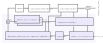
\includegraphics[width = 0.99\textwidth]{fig_C2_PBAdiagram.tex}
    \caption{Schematic diagram of the passivity-based adaptive controller (PBAC), where $\Sigma_{\textrm{softrobot}}$ denotes the dynamical system \eqref{eq:C2:dynamic_model} and $\Sigma_{\textrm{sensor}}$ a system of sensors suitable of measuring $\q$ and $\dq$. }
    \label{fig:C2:PBA_diagram}
  \end{figure}


\noindent where $\dq_r = \dq_d - \LambdaB \eB $ is called the reference velocity vector, $\LambdaB \in \R^{n \times n}$ a positive diagonal matrix, and $\vec{Y}(\q,\dq,\dq_r,\dq_r,\piB) \in \R^{m\times n}$ is called the regressor matrix. Following the work of Slotine and Li \cite{Slotine1988}, the control law and adaptation law are given by
%
\begin{align}
\tauB = &\, \tmat{M}\,\ddq_r + \tmat{C}\, \dq_r + \tvec{f}\!\grav +  \tvec{f}\!\elastic - \tvec{\delta} - \mat{K}_p \, \vec{e} - \mat{K}_d\, \vec{e}_r,  \label{eq:C2:tau} \\
\dot{\tvec{\pi}} =& - \mat{K}_{\vec{\pi}}\,\vec{Y}^\top\vec{e}_r,  \label{eq:C2:update}
\end{align}
%
where $\vec{e}_r := \dq - \dq_r = \dot{\vec{e}} + \LambdaB\,\vec{e}$, $\mat{K}_p, \mat{K}_d \in \mathbb{R}^{n\times n}$ are controller gains, and $\mat{K}_{\vec{\pi}} \in \R^{p\times p}$ is a positive definite matrix called the adaptation rate. Since $\tauB$ define the desired generalized forces acting on the system \eqref{eq:C2:dynamic_model}, the desired pressures are computed as $\uB = \mat{G}^{+} \tauB$ with $\mat{G}^{+}$ the generalized inverse of $\mat{G}$. A schematic diagram of the passivity-based controller is provided in Figure \ref{fig:C2:PBA_diagram}. It should be mentioned that the magnitude of adaptation rate does not affect the global stability of the system (if unmodelled dynamics are not excited); however, it sets the rate of adaptation, and accordingly the performance of the system.

\begin{rmk}[Persistence of excitation]
\label{rmk:C2:poe}
\editl It is important to note that the convergence of the tracking error $\eB \to 0$ does not imply convergence of the estimated parameter to their true values. According to \cite{Slotine1988,Slotine1989Jul,SlotineJ1987}, asymptotic convergence can be shown if the matrix $\vec{Y}(\q,\dq,\dq_r,\dq_r,\piB)$ is persistently excited and it is uniformly continuous. To elaborate, under the condition of persistent excitation, that is, for any instances $t_1,t_2$ with  $t_1\le t_2$  there exists a positive constant $\alpha$ such that $\int_{t_1}^{t_2} \mat{Y}^\top\,\mat{Y} \;dt \preceq \alpha\,\mat{I}$, it can be proven that the parameter estimates converge asymptotically to their true values. The authors in \cite{Slotine1988} state that the proof for convergence here applied to nonlinear robot dynamics is similar to those of linear dynamics \cite{Morgan1977} although the proof is fairly involved. \editr
\end{rmk}
%
